% "{'classe':('PSI'),'chapitre':'dyn_cin','type':('td'),'titre':'Culbuto', 'source':'Équipe PT - La Martinière Monplaisir','comp':('C1-05','C2-09'),'corrige':False}"
%\setchapterimage{bandeau}
\chapter*{Colle \arabic{cptColle} \\ 
Culbuto -- \ifprof Corrigé \else Sujet \fi}
\addcontentsline{toc}{section}{Colle \arabic{cptColle} : Culbuto -- \ifprof Corrigé \else Sujet \fi}

\iflivret \stepcounter{cptColle} \else
\ifprof  \stepcounter{cptColle} \else \fi
\fi

\setcounter{question}{0}
\marginnote{Équipe PT -- PT$\star$ La Martinière Monplaisir.}
\marginnote{
\UPSTIcompetence[2]{C1-05}
\UPSTIcompetence[2]{C2-09}
}



\begin{marginfigure}
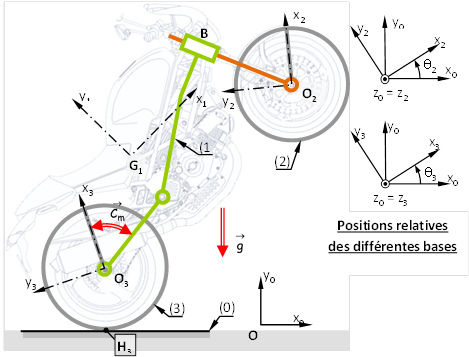
\includegraphics[width=\linewidth]{fig_01}
\end{marginfigure}
Le schéma de la figure ci-contre représente un jouet d’enfant constitué d’un premier solide \textbf{(1)}, assemblage d’un demi disque de rayon $R_1$ et d’une tige, et d’un solide \textbf{(2)}, guidé par une glissière de centre $A$ sur la tige de \textbf{(1)}.
Un ressort \textbf{(r)}, de raideur $k$ et de longueur libre $L_0$, est interposé entre les deux solides.
Le disque \textbf{(1)} est en contact ponctuel en $H$ avec le sol \textbf{(0)}. On suppose qu’il y a roulement sans glissement en $H$ entre \textbf{(0)} et \textbf{(1)}.

\textbf{Paramétrage et éléments d'inertie}
\begin{itemize}
\item Le repère $\repere{O}{x_0}{y_0}{z_0}$ lié au bâti est supposé galiléen. Le repère $\repere{C}{x_1}{y_1}{z_1}$ est lié au disque \textbf{(1)}.
\item La liaison glissière entre \textbf{(1)} et \textbf{(2)} est supposée sans frottement.
\item On note : $\angl{x_0}{x_1}=\angl{y_0}{y_1}=\theta_1$, 
$\vect{CA}=\lambda_2\vect{y_1}$, 
$\vect{HC}=R_1\vect{y_0}$,  
$\vect{CG_1}=-a_1\vect{y_1}$,
$\vect{AG_2}=a_2\vect{y_1}$.
\item \textbf{(1)} : masse $m_1$, $\inertie{G_1}{1}=\matinertie{A_1}{B_1}{C_1}{0}{0}{0}{\mathcal{B}_1}$;
\item \textbf{(2)} : masse $m_2$, $\inertie{G_2}{2}=\matinertie{A_2}{B_2}{C_2}{0}{0}{0}{\mathcal{B}_2}$
\end{itemize}.

\question{Déterminer les équations différentielles du mouvement de \textbf{(1)} et de \textbf{(2)} par rapport au bâti \textbf{(0)}.}


\ifprof
\else
\begin{marginfigure}
\centering

\includegraphics[width=3cm]{Cy_04_02_Colle_PFD_01_Culbuto_qr}
\end{marginfigure}
\fi



